\newpage
\section{Turn Up the Volume!}

In this activity, we will investigate formulas for area and
volume.


\begin{prob}
Explain how the following picture ``proves'' that the area of a right
  triangle is one half of the base times the height.
\[
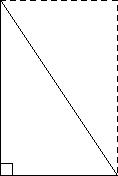
\includegraphics{../graphics/pbpAreaRight.pdf}
\]
\end{prob}


\begin{prob}
``Shearing'' is a process where you take a shape, cut it into thin strips, 
then push the strips around in one direction to make a new shape.  
Cavalieri's principle states:\index{Cavalieri's principle}
\begin{quote}
Shearing parallel to a fixed direction does not change the
$n$-dimensional measure of an object.
\end{quote}
What is this saying?
\end{prob}




\begin{prob}
Building on the first two problems, explain how the following picture
  ``proves'' that the area of any triangle is one half of the base times the
  height.
\[
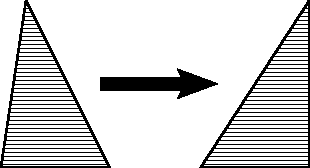
\includegraphics{../graphics/pbpShearTri.pdf}
\]
\end{prob}




\begin{prob}
Give an intuitive argument explaining why Cavalieri's principle is
true.
\end{prob}


\begin{prob}
Explain how to use a picture to ``prove'' that a triangle of a given
  area could have an arbitrarily large perimeter.
\end{prob}


%
%\begin{prob}
%Sketch a net for a right pyramid of height $2''$ with a $2'' \times
%2''$ square base. Share your sketch with your neighbor---does it look
%OK?
%\end{prob}
%
%
%\begin{prob}
%Give detailed diagrams that show that a cube can be constructed from
%three equal pyramids.
%\end{prob}

\begin{prob}
Cut out the provided net.  Then fold it and tape it to create a square-based pyramid.  With your neighbors, show that three such square-based pyramids can form a cube.  
\end{prob}
\begin{teachingnote}
Here is the net
$$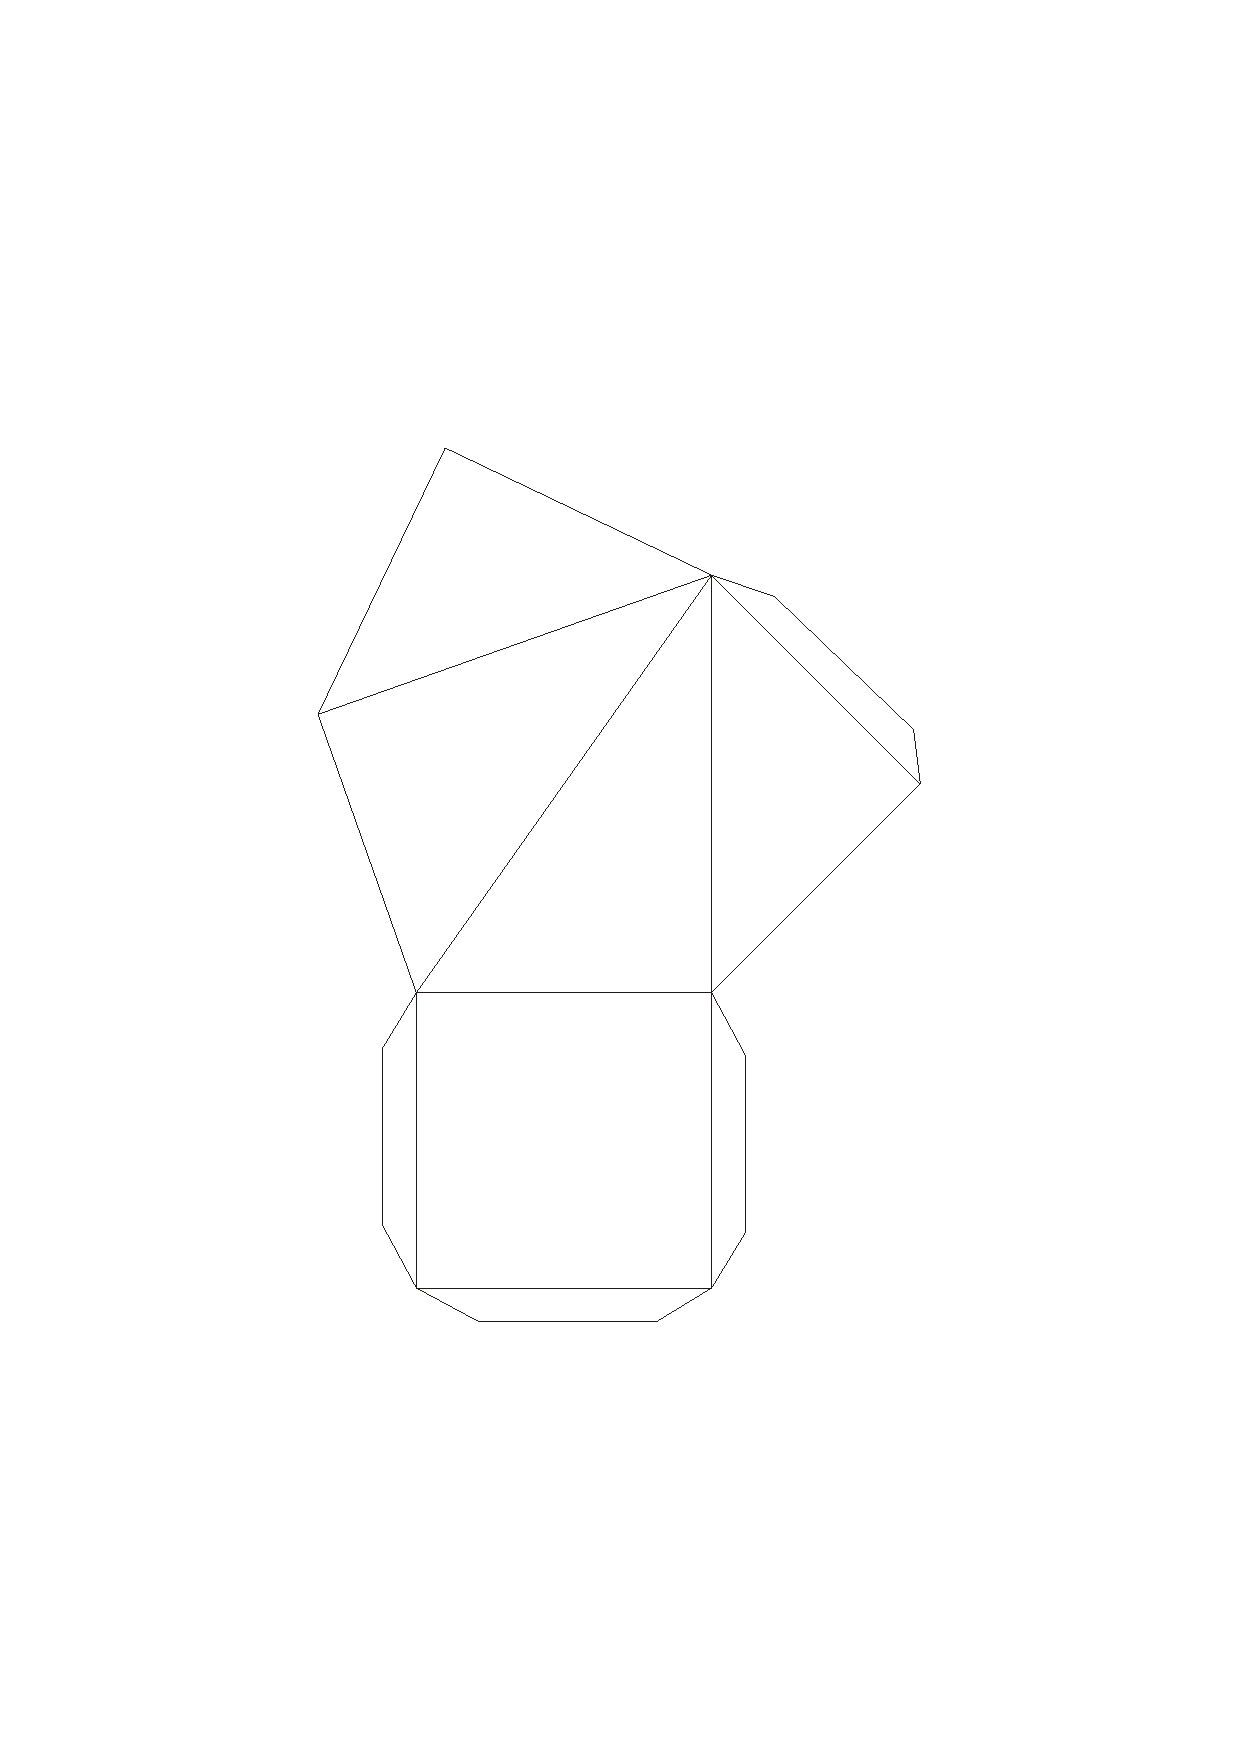
\includegraphics[angle=90,scale=0.7]{../graphics/rightPyramid}$$
\end{teachingnote}

\begin{prob}
Use your work above to derive a formula for the volume of a
right pyramid with a square base. The formula should be in terms of
the side length of the square base.
\end{prob}

\begin{prob}
Use Cavalieri's principle to explain the formula for \textbf{every} pyramid with an $s\times s$ square base of height $s$ in terms of $s$.  Be sure to describe how this formula is different from the previous one.  
\end{prob}

\begin{prob}
Provide an informal explanation of a volume formula for any pyramid-like object with a base of area $B$ and height $h$.  Be sure to describe what you mean by ``pyramid-like'' and whether your formula works for a cone.  
\end{prob}

\begin{prob}
Answer the following question using the provided figure showing cross-sections at height $h$ of a half-sphere and and of a cylinder with a cone inside it.\standard{8.G.9}\standardhs{G-GMD.1}\standardhs{G-GMD.2}  
\begin{enumerate}
\item Explain why the two colored cross-sections at height $h$ have the same area. 
\item Use the formula for the volume of a cone and Cavalieri's principle to derive a formula for the radius of a sphere of radius $r$.  
\end{enumerate}
\end{prob}

\begin{teachingnote}
Here is the figure:  
$$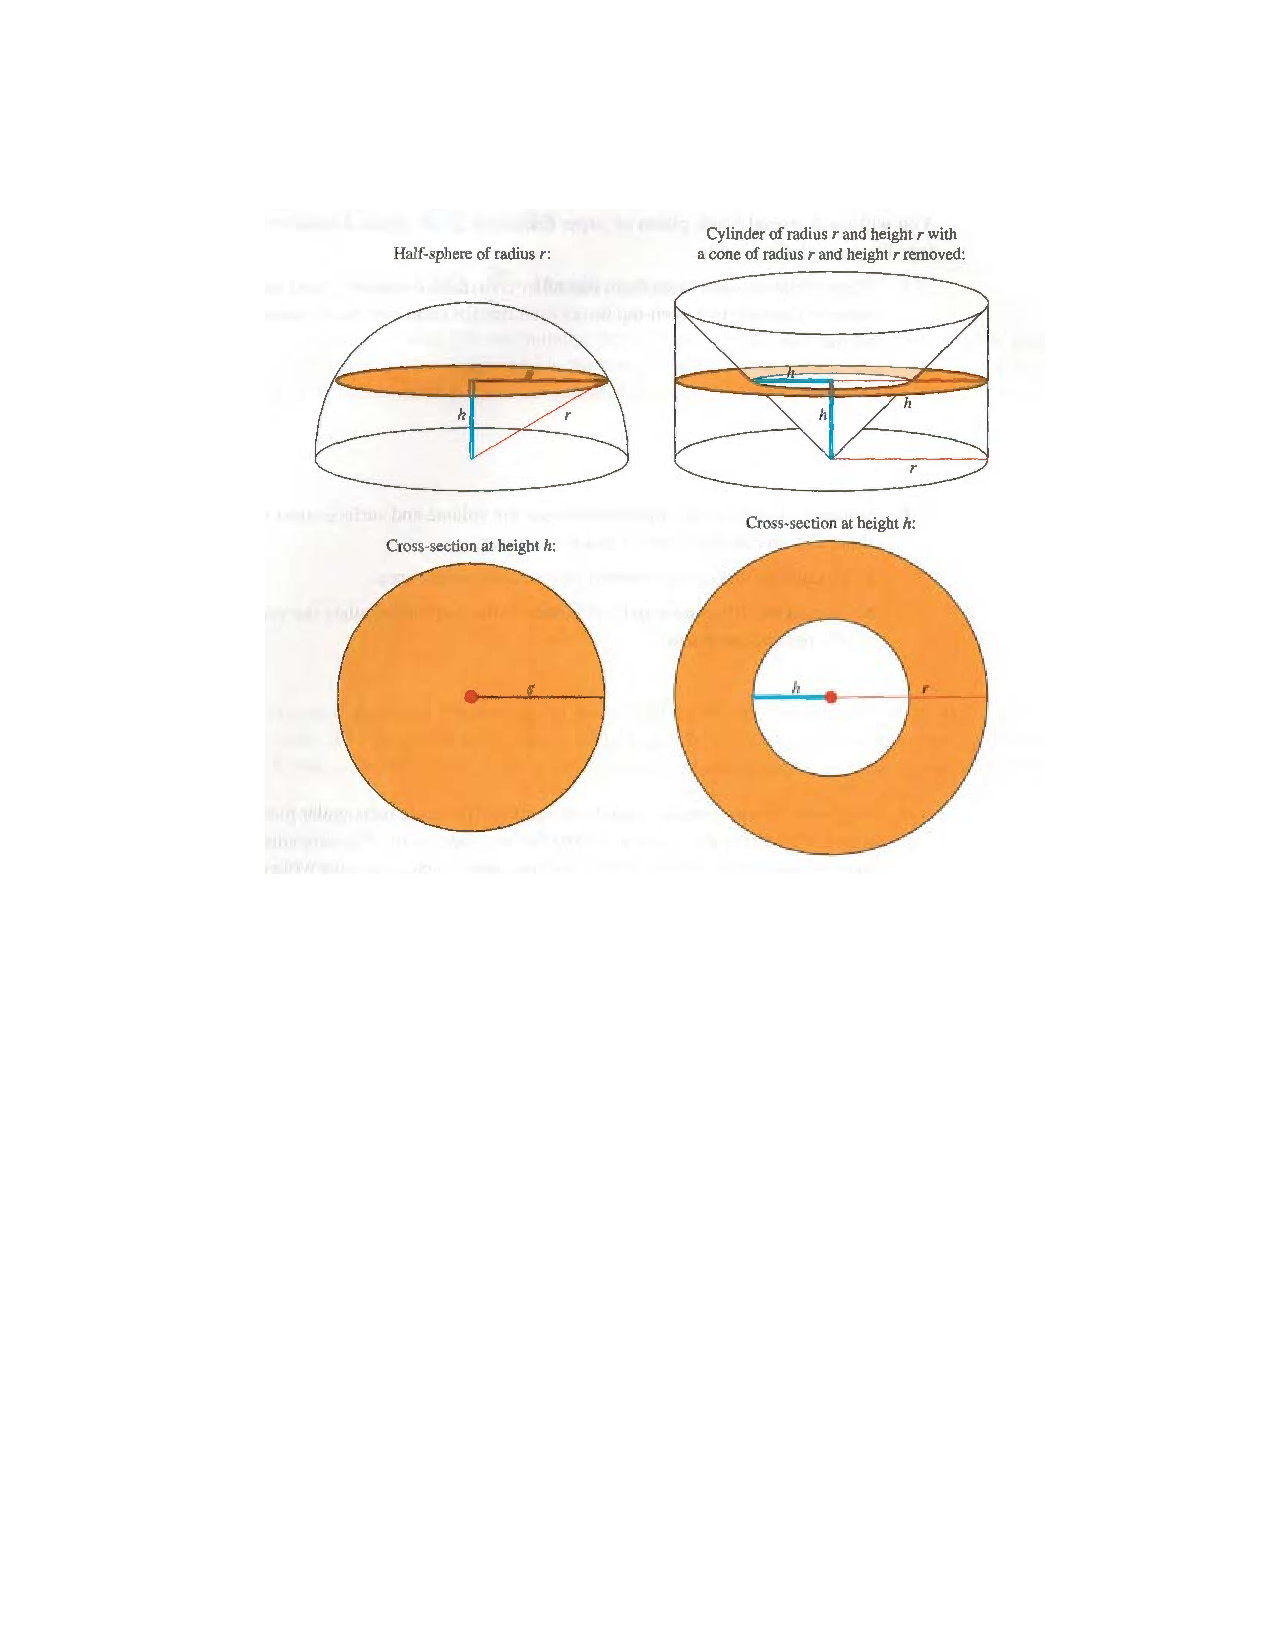
\includegraphics{../graphics/sphereVolume}$$
\end{teachingnote}

